\section{Цепь №1 (<<Масштабный усилитель с инверсией фазы>>)}

\sidefig(0.5\textwidth){
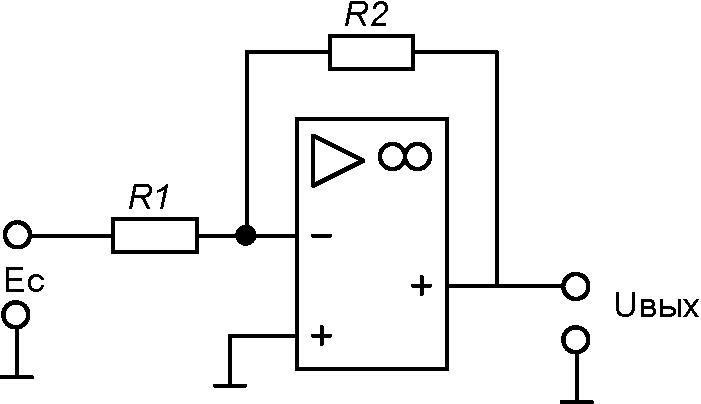
\includegraphics[scale=0.6]{Circ1.pdf}
\caption{Схема}
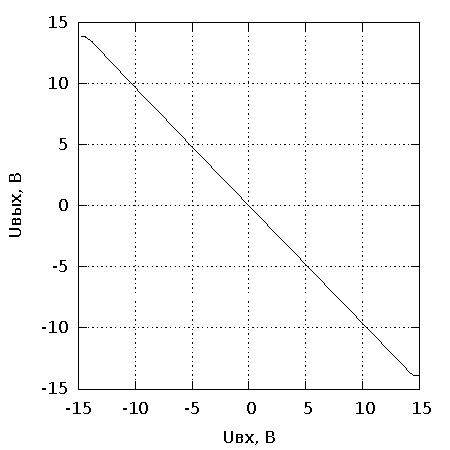
\includegraphics[scale=1.2]{1.pdf}
\caption{Для постоянного тока}}
{Табл. 1: Для постоянного тока

\small
\begin{tabular}{|l|l|l|}
\hline
$U_{вх}$, В & $U_{вых}$, В & K \\
\hline
-14.72&13.82&0.94\\
\hline
-14.56&13.82&0.95\\
\hline
-14.45&13.82&0.96\\
\hline
-14.24&13.69&0.96\\
\hline
-13.8&13.4&0.97\\
\hline
-12.6&12.2&0.97\\
\hline
-10.99&10.6&0.96\\
\hline
-8.62&8.28&0.96\\
\hline
-7.86&7.6&0.97\\
\hline
-6.54&6.28&0.96\\
\hline
-5.1&4.9&0.96\\
\hline
-3.73&3.58&0.96\\
\hline
-2.43&2.33&0.96\\
\hline
-1.3&1.25&0.96\\
\hline
0.11&-0.104&0.95\\
\hline
0.15&-0.14&0.93\\
\hline
1.07&-1.03&0.96\\
\hline
2.57&-2.47&0.96\\
\hline
3.29&-3.16&0.96\\
\hline
4.42&-4.24&0.96\\
\hline
5.78&-5.55&0.96\\
\hline
6.79&-6.53&0.96\\
\hline
7.62&-7.31&0.96\\
\hline
8.12&-7.82&0.96\\
\hline
8.59&-8.25&0.96\\
\hline
9.21&-8.84&0.96\\
\hline
9.9&-9.51&0.96\\
\hline
10.91&-10.48&0.96\\
\hline
11.51&-11.06&0.96\\
\hline
12.29&-11.8&0.96\\
\hline
13.64&-13.1&0.96\\
\hline
14.2&-13.68&0.96\\
\hline
14.33&-13.76&0.96\\
\hline
14.5&-13.89&0.96\\
\hline
14.79&-13.91&0.94\\
\hline
14.97&-13.9&0.93\\
\hline
\end{tabular}}

\sidefig(0.5\textwidth){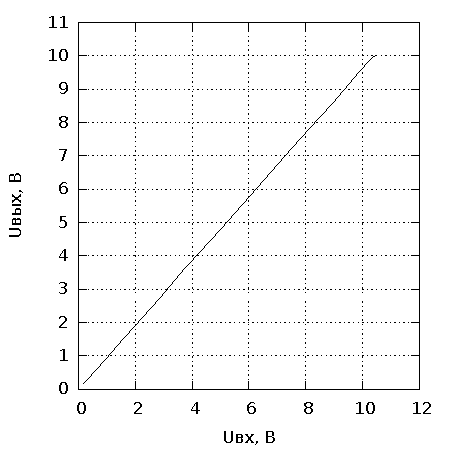
\includegraphics[scale=1.2]{2.pdf}
\caption{Для переменного тока}}
{Табл. 2: Для переменного тока

\begin{tabular}{|l|l|l|}
\hline
$U_{вх}$, В & $U_{вых}$, В & K \\
\hline
0.17&0.16&0.94\\
\hline
0.59&0.56&0.95\\
\hline
1.02&0.97&0.95\\
\hline
1.59&1.53&0.96\\
\hline
1.82&1.74&0.96\\
\hline
2.92&2.79&0.96\\
\hline
3.61&3.5&0.97\\
\hline
4.95&4.74&0.96\\
\hline
5.96&5.72&0.96\\
\hline
7.57&7.28&0.96\\
\hline
8.31&7.98&0.96\\
\hline
8.99&8.61&0.96\\
\hline
9.51&9.13&0.96\\
\hline
9.72&9.35&0.96\\
\hline
10.31&9.92&0.96\\
\hline
10.5&10.02&0.95\\
\hline
\end{tabular}}

Табл. 3: Зависимость K от $R_1$ и $R_2$

\begin{tabular}{|l|l|l|l|l|l|}
\hline
$R_1$, Ом & $R_2$, Ом & $U_{вх}$, В & $U_{вых}$, В & $K_{теор}$ & $K_{эксп}$ \\
\hline
51&100&0.36&0.64&1.96&1.78\\
\hline
100&200&0.68&1.29&2.00&1.90\\
\hline
5100&10000&2.55&4.94&1.96&1.94\\
\hline
10000&20000&2.54&5.28&2.00&2.08\\
\hline
20000&40000&2.97&5.69&2.00&1.92\\
\hline
50000&100000&2.5&5.37&2.00&2.15\\
\hline
\end{tabular}
\begin{figure}[H]
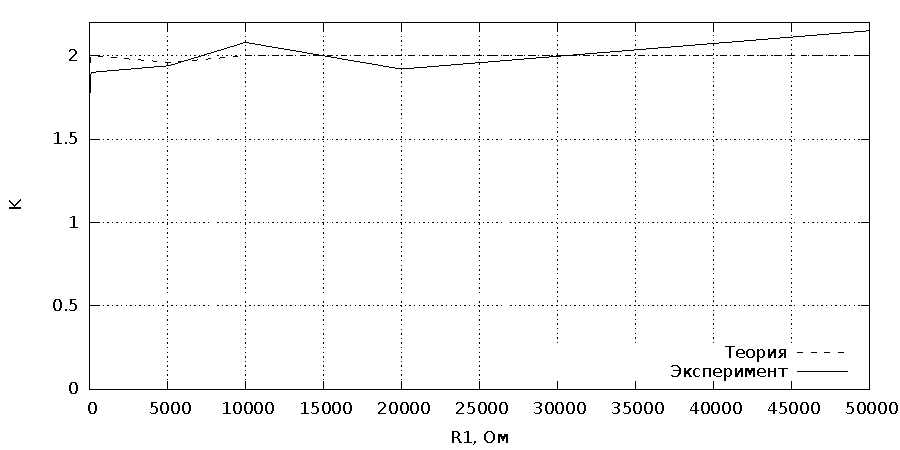
\includegraphics[scale=1]{3.pdf}
\caption{Коэффициент усиления}
\end{figure}